% This is samplepaper.tex, a sample chapter demonstrating the
% LLNCS macro package for Springer Computer Science proceedings;
% Version 2.20 of 2017/10/04
%
\documentclass[runningheads]{llncs}
%
\usepackage{graphicx}
% Used for displaying a sample figure. If possible, figure files should
% be included in EPS format.
%
% If you use the hyperref package, please uncomment the following line
% to display URLs in blue roman font according to Springer's eBook style:
% \renewcommand\UrlFont{\color{blue}\rmfamily}

\begin{document}
%
\title{Subtle Gestures with the J!NS MEME}
%
%\titlerunning{Abbreviated paper title}
% If the paper title is too long for the running head, you can set
% an abbreviated paper title here
%
\author{Thomas Bartel \and
Florian Bossert \and
Sajjad Ahmad}
%
% TODO should we use 'et al.' here? ~FB
\authorrunning{T. Bartel \and F. Bossert \and S. Ahmad}
% First names are abbreviated in the running head.
% If there are more than two authors, 'et al.' is used.
%
\institute{Karlsruhe Institute of Technology, Karlsruhe, Germany}
%
\maketitle              % typeset the header of the contribution
%
\begin{abstract}
The abstract should briefly summarize the contents of the paper in
15--250 words.

\keywords{First keyword  \and Second keyword \and Another keyword.}
\end{abstract}
%
%
%
\section{Introduction}
\subsection{A Subsection Sample}
Please note that the first paragraph of a section or subsection is
not indented. The first paragraph that follows a table, figure,
equation etc. does not need an indent, either.

Subsequent paragraphs, however, are indented.

% As a reference, maybe useful later
Current smartglasses:
Smartglasses with cameras: Spectacles by Snap Inc. https://www.spectacles.com/
Smartglasses with EOG sensors: J!ns Meme by J!ns (website currently only in Japanese):
https://jins-meme.com/

% Assigned to FB
\section{Related Work}
Our work touches on multiple areas of research, including wearable sensing, gesture
recognition, and subtle interaction. In the following section we roughly outline
previous works in these areas.

\subsection{The Human Body as an Input Interface}
There are various works discussing the use of the human body as an input interface, with
most of them having an exploratory nature:
Harrison et al. resolved the location of finger tapping on the user's arm and hand
using acoustic sensing \cite{10.1145/1753326.1753394}.
Serrano et al. explored Hand-to-Face input by tracking infrared markers applied to
fingers with an optical system \cite{10.1145/2556288.2556984}.
Lisserman et al. proposed the human ear as an input surface, which can be used by
touching it in certain ways. This was achieved by placing electrodes around the ear
\cite{10.1145/2468356.2468592}.
Even eyelid gestures have been looked into by Jota et al., who developed a framework
and prototypes for them \cite{10.5555/2788890.2788938}.
Using a battery-free low-power wrist band, Truong et al. managed to classify hand
gestures by detecting skin deformations \cite{10.1145/3274783.3274854}.

Especially when using extremities as input methods, inertial measurement units (IMUs),
which consist of accelerometers and gyroscopes, have been widely employed: Wen et al.
used them to recognize unremarkable fine-motor finger movements
\cite{10.1145/2858036.2858466}. Laput et al. utilized the IMUs in commercially available
smartwatches with a custom performance-boosting kernel to classify a wide variety of hand
gestures \cite{10.1145/2984511.2984582}.

As for applications of wearable sensing, there are many from convenient user input
to medical monitoring:
Ike et al. demonstrated using hand gestures to control a TV's content navigation interface
with a IMU-equipped wrist band \cite{10.1145/2641248.2641359}.
Ohnishi et al. used sensors in shoes to track exercises and general posture
\cite{10.1145/3174910.3174938}.
Schiboni et al. monitored drinking with wrist-worn inertial sensors, demonstrating
the feasibility of long-term sparse natural gesture recognition
\cite{10.1145/3267242.3267253}.
On the more medical side, Milosevic et al. performed jump performance analysis with
low-cost wearable devices instead of pressure-sensitive force plates, with the intent
of making training progress monitoring more easily available \cite{10.1145/2753509.2753512}.
Again for automatic monitoring, Bedri et al. used wearable sensors to track
eating episodes instead of making patients rely on often biased self-written food intake
journals \cite{10.1145/3130902}.

\subsection{EOG Sensing and Subtle Interaction}
While the aforementioned work utilized mainly IMUs, touch sensors or optical systems,
Electrooculography (EOG) has become a useful tool for eye-tracking in recent years, too. 
In 2006, Manabe et al. attached EOG sensors to over-ear \cite{10.1145/1125451.1125655}
and in 2013, to in-ear head phones \cite{10.1145/2493988.2494329} to detect eye gestures.
Bulling et al. first demonstrated efficient real-time eye-movement recognition
with EOG goggles in 2009, which they custom-made \cite{10.1145/1520340.1520468}.
Once commercial EOG glasses became available in 2014, Ichimaru et al. used them for
activity recognition \cite{10.1145/2638728.2638795}. They used the J!ns Meme
smartglasses to distinguish between typing, reading, eating and talking.
As for more recent work, Li et al. used the J!ns Meme to infer the physical and social
context of the wearer by recognizing various greeting gestures involving kissing
\cite{10.1145/3384657.3384801}.

In contrast to the work discussed, which often employed noticable or obviously unusual
hardware, we explicitly focus on subtle interaction. Pohl et al. define
four types of subtle interaction: (1) signifying feedback that is non-intrusive to the
user, (2) hiding interaction from others and potentially deceiving them, (3) employing
less effort for input and generally doing less, and (4) nudging users
\cite{10.1145/3290605.3300648}. Our work aims at type (2) social subtlety, like e.g.
Ashbrook et al. did with their tooth-click gesture recognition interface
\cite{10.1145/2935334.2935389}. With a similar goal, Li et al. developed TongueBoard,
a retainer form-factor device for recognizing silent speech \cite{10.1145/3311823.3311831}.

Itchy Nose by Lee et al. is the most closely related work to ours,
as it inspired our efforts \cite{10.1145/3123021.3123060}. They used the J!ns Meme
smartglasses to detect multiple gestures that consisted of rubbing or pushing their
noses, which can also be detected by the glasses' EOG sensors.

% Assigned to FB
\section{Analysis}
% TODO introduction for analysis section
What does our research contribute? (Additional subtle gestures, ...)

% TODO, maybe do this in the Introduction section? ~FB
Explaining the J!ns Meme.

% TODO
What was our goal?

\subsection{Workflow}
We began with planning the rough outline that our research would follow.
The plan was as follows:
\begin{itemize}
    \item Gather gesture ideas
    \item Check ideas for detectable responses
    \item Create tools to automate the recording of gestures
    \item Collect labelled data with the tools
    \item Model, train and validate a neural network until its performance is sufficient
    \item Test the network on our withheld test dataset
\end{itemize}

[Insert figure here]

\subsection{Gestures}
% TODO, maybe use self-made illustrations here
In the first phase, we came up with gestures we considered subtle. Early candidates were:
\begin{itemize}
    \item Pushing your glasses up your nose [see GIF]
    \item A thinking pose, where you touch your chin with your thumb and your cheek with your
        index finger [see GIF]
    \item Slow nodding [see GIF]
    \item Tapping the frame of the glasses [see GIF]
\end{itemize}

Since some of the gestures generated barely any responses on the EOG or the IMU readouts
[see figures with an example of a strong and a weak response],
we continued coming up with gestures until we had a total of seven gestures.
The gestures we came up with and their apparent responses can be seen in table \ref{responses}.

\begin{table}
\caption{The quality of the EOG and IMU sensor responses for our gestures.}\label{responses}
\begin{tabular}{|l|l|}
    \hline
    Gesture description & Response quality\\
    \hline
    Pushing glasses up the nose & strong\\
    Readjusting glasses & strong\\
    Thinking pose & weak\\
    Slow nodding & strong\\
    Tilting head sideways & strong\\
    Stroking mustache & weak\\
    Biting lip & weak\\
    Tapping on the nose & strong\\
    Rubbing the nose & strong\\
    Pushing cheek up with a finger & strong\\
    Tapping the glasses & strong\\\hline
\end{tabular}
\end{table}

\subsection{Tools for Recording and Labelling}
% is this something for the implementation section? ~FB
How does the J!ns Meme work and how do we use it?

What data do we collect, how and why?
Itchy Nose tool for automating personalization \cite{10.1145/3174910.3174953}.

\subsection{Neural Network Architecture and Training}
% again - how much of this belongs to implementation? ~FB

% Assigned to TB
\section{Implementation}
\subsection{A Subsection Sample}
Please note that the first paragraph of a section or subsection is
not indented. The first paragraph that follows a table, figure,
equation etc. does not need an indent, either.

Subsequent paragraphs, however, are indented.

% Assinged to SA
\section{Results}
\subsection{A Subsection Sample}
Please note that the first paragraph of a section or subsection is
not indented. The first paragraph that follows a table, figure,
equation etc. does not need an indent, either.

Subsequent paragraphs, however, are indented.

% Assigned to TB
\section{Discussion}
\subsection{A Subsection Sample}
Please note that the first paragraph of a section or subsection is
not indented. The first paragraph that follows a table, figure,
equation etc. does not need an indent, either.

Subsequent paragraphs, however, are indented.

\section{Future Work}
\subsection{A Subsection Sample}
Please note that the first paragraph of a section or subsection is
not indented. The first paragraph that follows a table, figure,
equation etc. does not need an indent, either.

Subsequent paragraphs, however, are indented.

\section{First Section}
\subsection{A Subsection Sample}
Please note that the first paragraph of a section or subsection is
not indented. The first paragraph that follows a table, figure,
equation etc. does not need an indent, either.

Subsequent paragraphs, however, are indented.

\subsubsection{Sample Heading (Third Level)} Only two levels of
headings should be numbered. Lower level headings remain unnumbered;
they are formatted as run-in headings.

\paragraph{Sample Heading (Fourth Level)}
The contribution should contain no more than four levels of
headings. Table~\ref{tab1} gives a summary of all heading levels.

\begin{table}
\caption{Table captions should be placed above the
tables.}\label{tab1}
\begin{tabular}{|l|l|l|}
\hline
Heading level &  Example & Font size and style\\
\hline
Title (centered) &  {\Large\bfseries Lecture Notes} & 14 point, bold\\
1st-level heading &  {\large\bfseries 1 Introduction} & 12 point, bold\\
2nd-level heading & {\bfseries 2.1 Printing Area} & 10 point, bold\\
3rd-level heading & {\bfseries Run-in Heading in Bold.} Text follows & 10 point, bold\\
4th-level heading & {\itshape Lowest Level Heading.} Text follows & 10 point, italic\\
\hline
\end{tabular}
\end{table}


\noindent Displayed equations are centered and set on a separate
line.
\begin{equation}
x + y = z
\end{equation}
Please try to avoid rasterized images for line-art diagrams and
schemas. Whenever possible, use vector graphics instead (see
Fig.~\ref{fig1}).

\begin{figure}
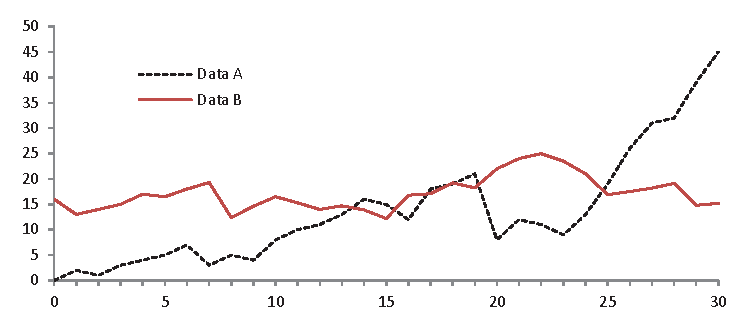
\includegraphics[width=\textwidth]{fig1.eps}
\caption{A figure caption is always placed below the illustration.
Please note that short captions are centered, while long ones are
justified by the macro package automatically.} \label{fig1}
\end{figure}

\begin{theorem}
This is a sample theorem. The run-in heading is set in bold, while
the following text appears in italics. Definitions, lemmas,
propositions, and corollaries are styled the same way.
\end{theorem}
%
% the environments 'definition', 'lemma', 'proposition', 'corollary',
% 'remark', and 'example' are defined in the LLNCS documentclass as well.
%
\begin{proof}
Proofs, examples, and remarks have the initial word in italics,
while the following text appears in normal font.
\end{proof}
For citations of references, we prefer the use of square brackets
and consecutive numbers. Citations using labels or the author/year
convention are also acceptable. The following bibliography provides
a sample reference list with entries for journal
% articles~\cite{ref_article1}, an LNCS chapter~\cite{ref_lncs1}, a
% book~\cite{ref_book1}, proceedings without editors~\cite{ref_proc1},
% and a homepage~\cite{ref_url1}. Multiple citations are grouped
% \cite{ref_article1,ref_lncs1,ref_book1},
% \cite{ref_article1,ref_book1,ref_proc1,ref_url1}.
%
% ---- Bibliography ----
%
% BibTeX users should specify bibliography style 'splncs04'.
% References will then be sorted and formatted in the correct style.
%
\bibliographystyle{splncs04}
\bibliography{mybibliography}
%
\end{document}
